\documentclass{beamer}
\usepackage[italian]{babel}
\usepackage{booktabs}
\usepackage{dirtytalk}


\usetheme{Luebeck}        
\useinnertheme{rectangles} 
\useoutertheme{tree} 
\usecolortheme{beaver} 
\usefonttheme{default}  

\addtobeamertemplate{navigation symbols}{}{%
    \usebeamerfont{footline}%
    \usebeamercolor[fg]{footline}%
    \hspace{1em}%
    \insertframenumber/\inserttotalframenumber}

\institute{Universit\`a di Bologna\\Corso di Laurea in Fisica}
\title[Chargino and neutralino production in final states]{iTHEPHY \\
Search for chargino and neutralino production in final states with a Higgs boson with the ATLAS detector}
\author{\textbf{Eric Ballabene},\\ \textbf{Massimiliano Gallli}}
\date{18 / 12 /2018}

\setbeamertemplate{headline}{} 

\begin{document}
\begin{frame}{}
\titlepage
\end{frame}


\begin{frame}{Analysis channels}
\vskip-0.2cm
\begin{figure}
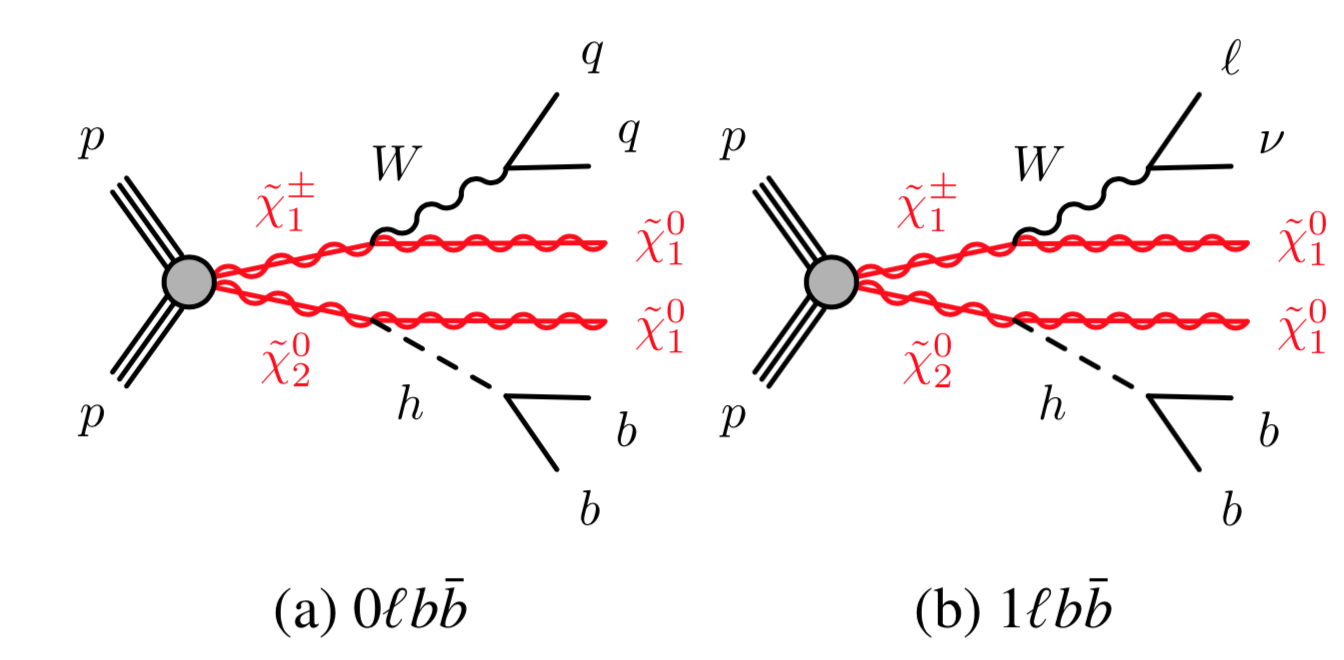
\includegraphics[width=0.72\textwidth]{fourchannel1}
\end{figure}
\begin{figure}
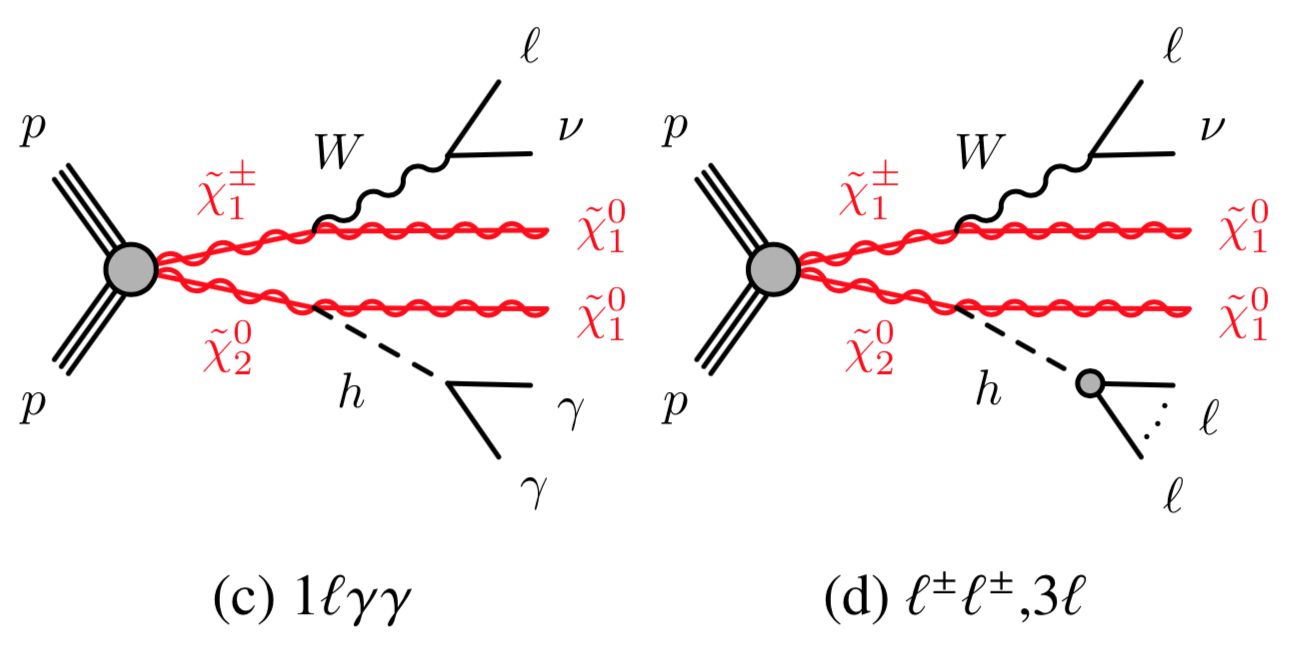
\includegraphics[width=0.72\textwidth]{fourchannel2}
\end{figure}
\end{frame}

\begin{frame}{Main backgrounds}
\begin{figure}[!h]
\centering
\begin{minipage}{.45\textwidth}
\centering
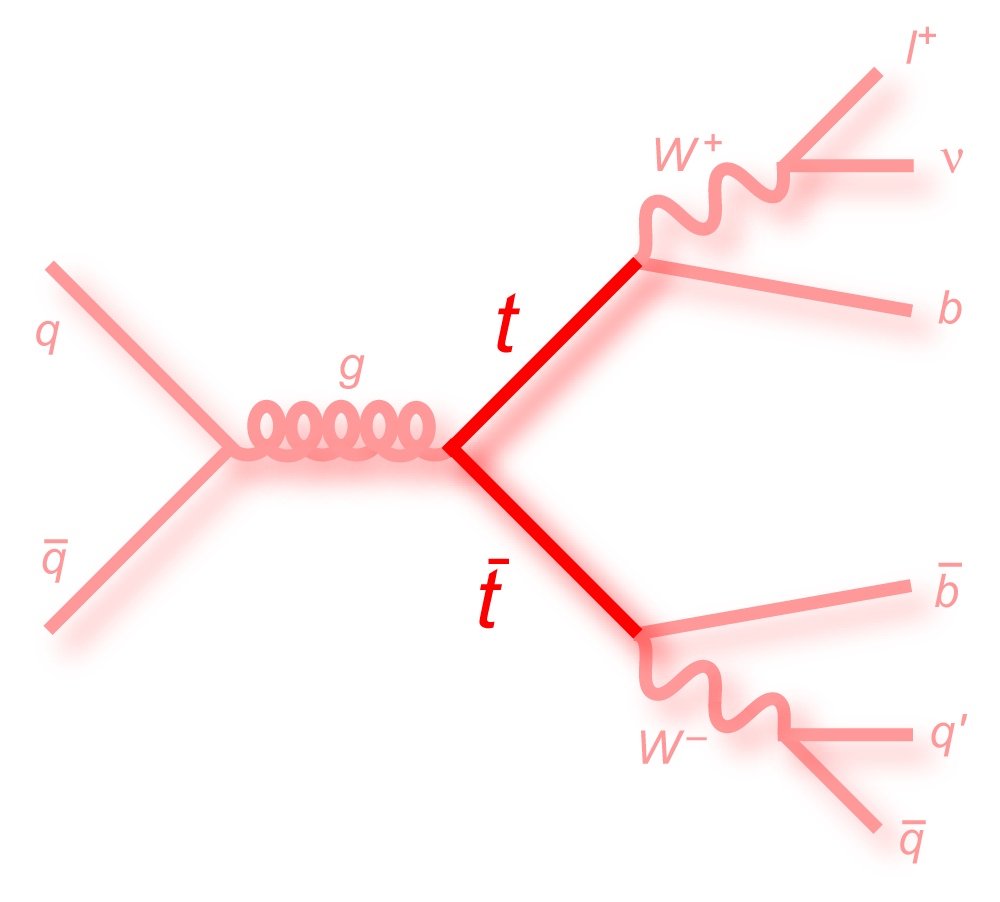
\includegraphics[height=0.8\textwidth,width=1.1\textwidth]{ttbar}
{\\(a) $t\bar{t}$}
\end{minipage}
\,\,\,\,\,\,\,\,
\begin{minipage}{.45\textwidth}
\centering
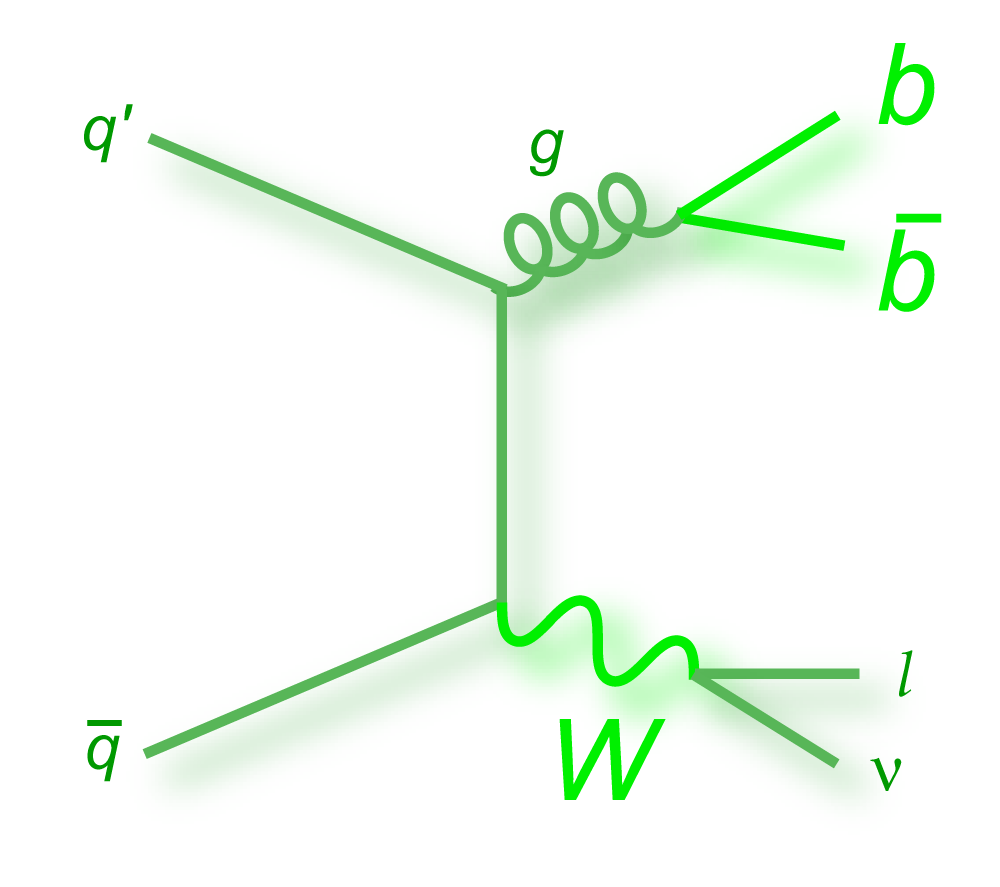
\includegraphics[height=0.8\textwidth,width=1.\textwidth]{w+jets}
{\\(b) $W+jets$}
\end{minipage}
\end{figure}
\end{frame}

\begin{frame}{Definition of the regions}
\begin{figure}
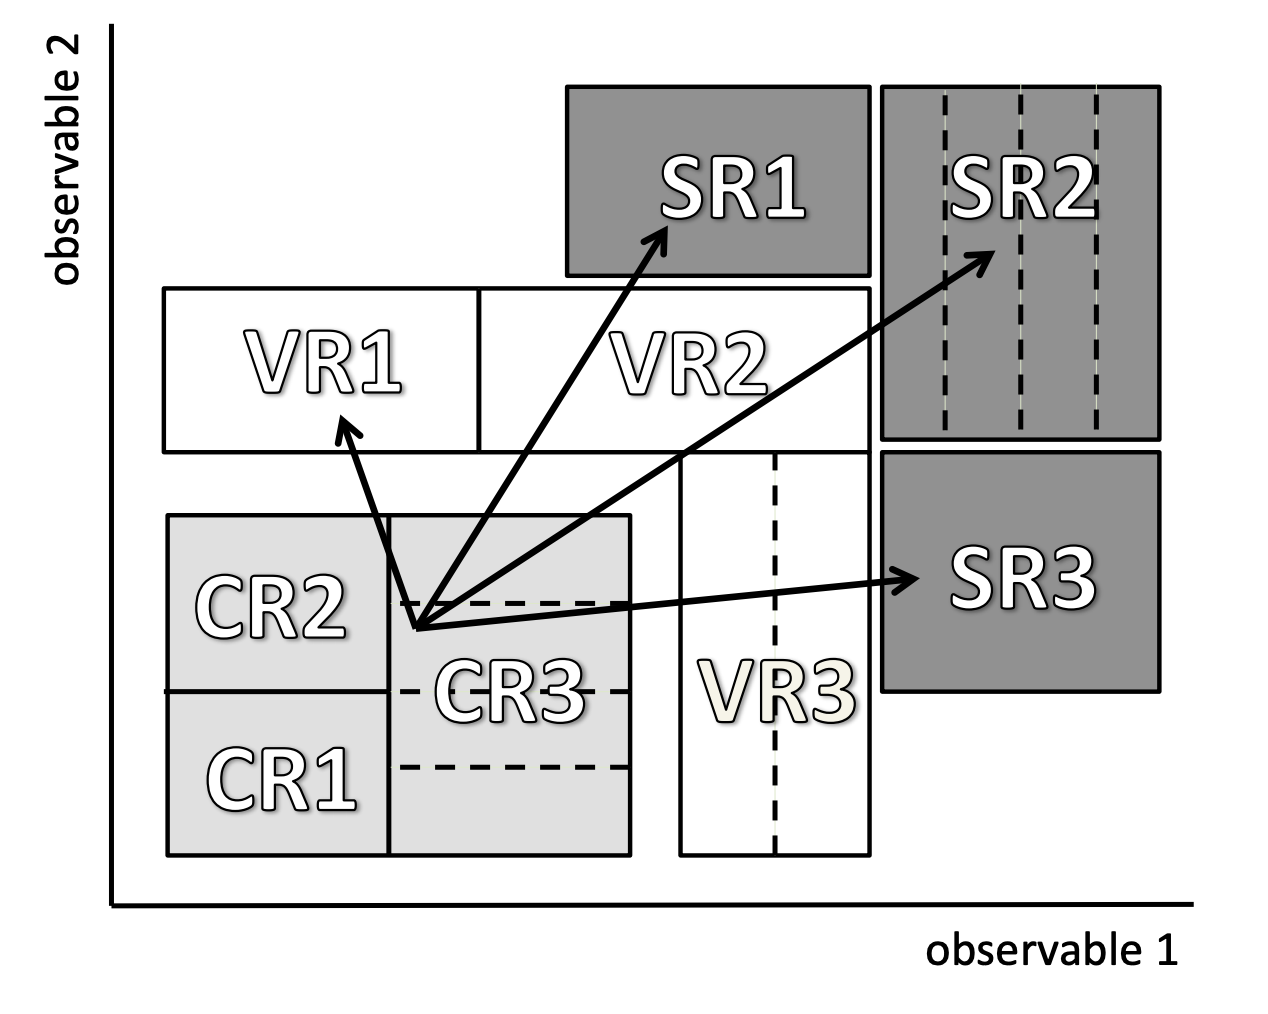
\includegraphics[width=0.75\textwidth]{regions}
\end{figure}
\end{frame}

\begin{frame}{Analysis flow}
\begin{figure}
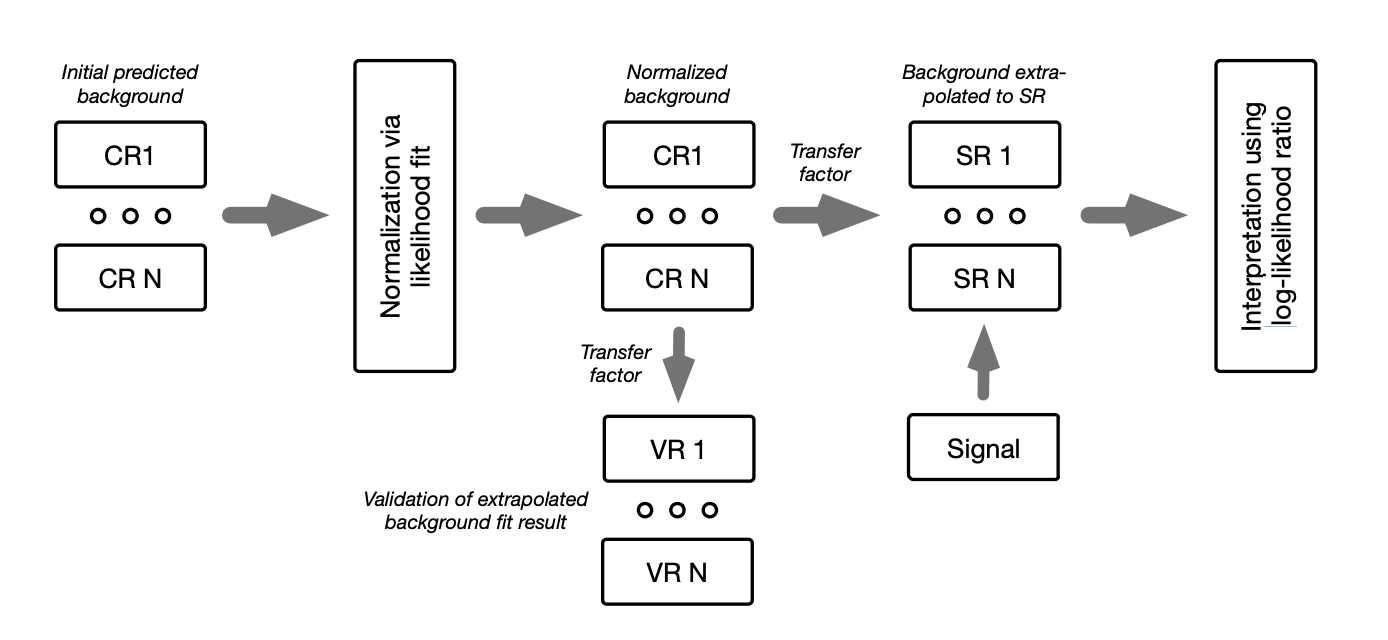
\includegraphics[width=1.\textwidth]{regions2}
\end{figure}
\end{frame}

\begin{frame}
\begin{columns}[onlytextwidth]
\begin{column}{.5\textwidth}
\begin{figure}
  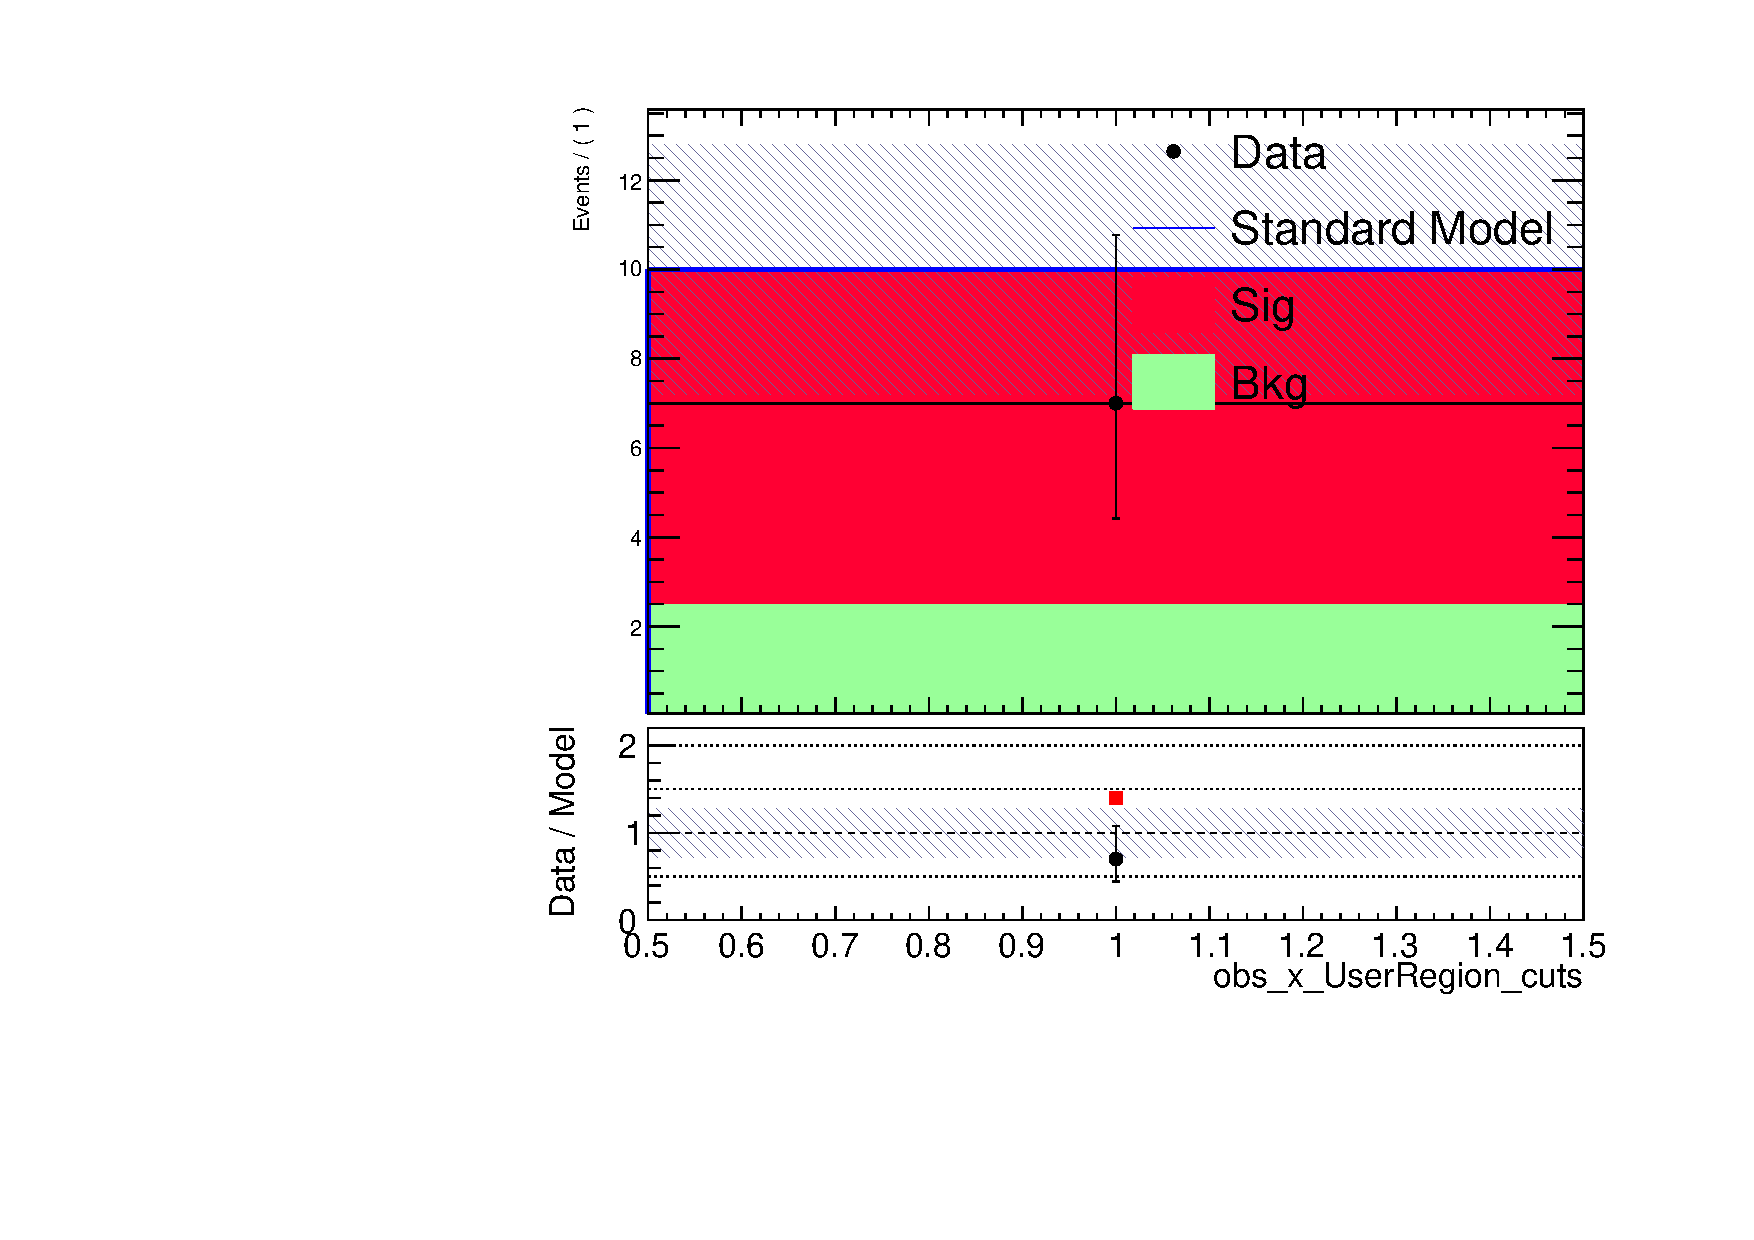
\includegraphics[width=\textwidth]{before}
\end{figure}
\end{column}
\begin{column}{.5\textwidth}
\begin{figure}
  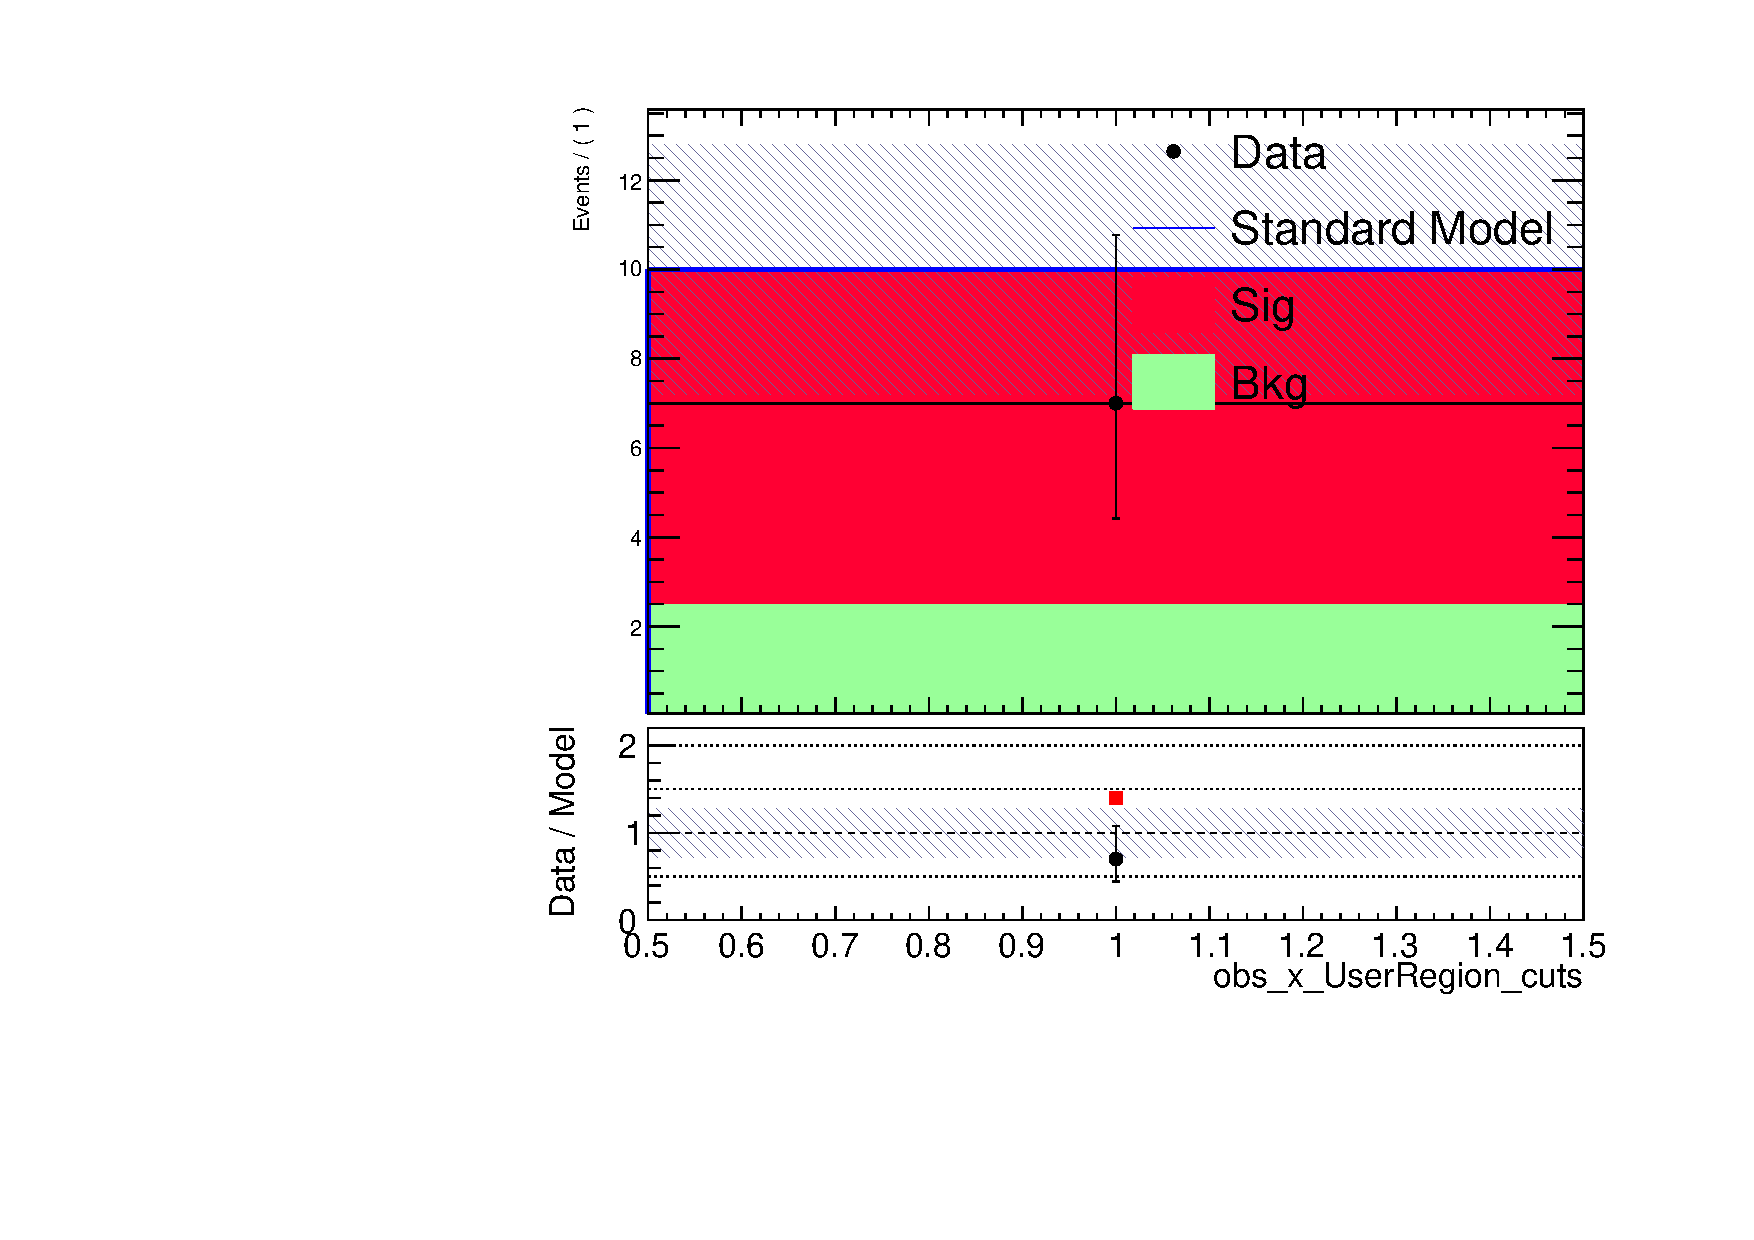
\includegraphics[width=\textwidth]{after}
\end{figure}
\end{column}
\end{columns}
\begin{figure}
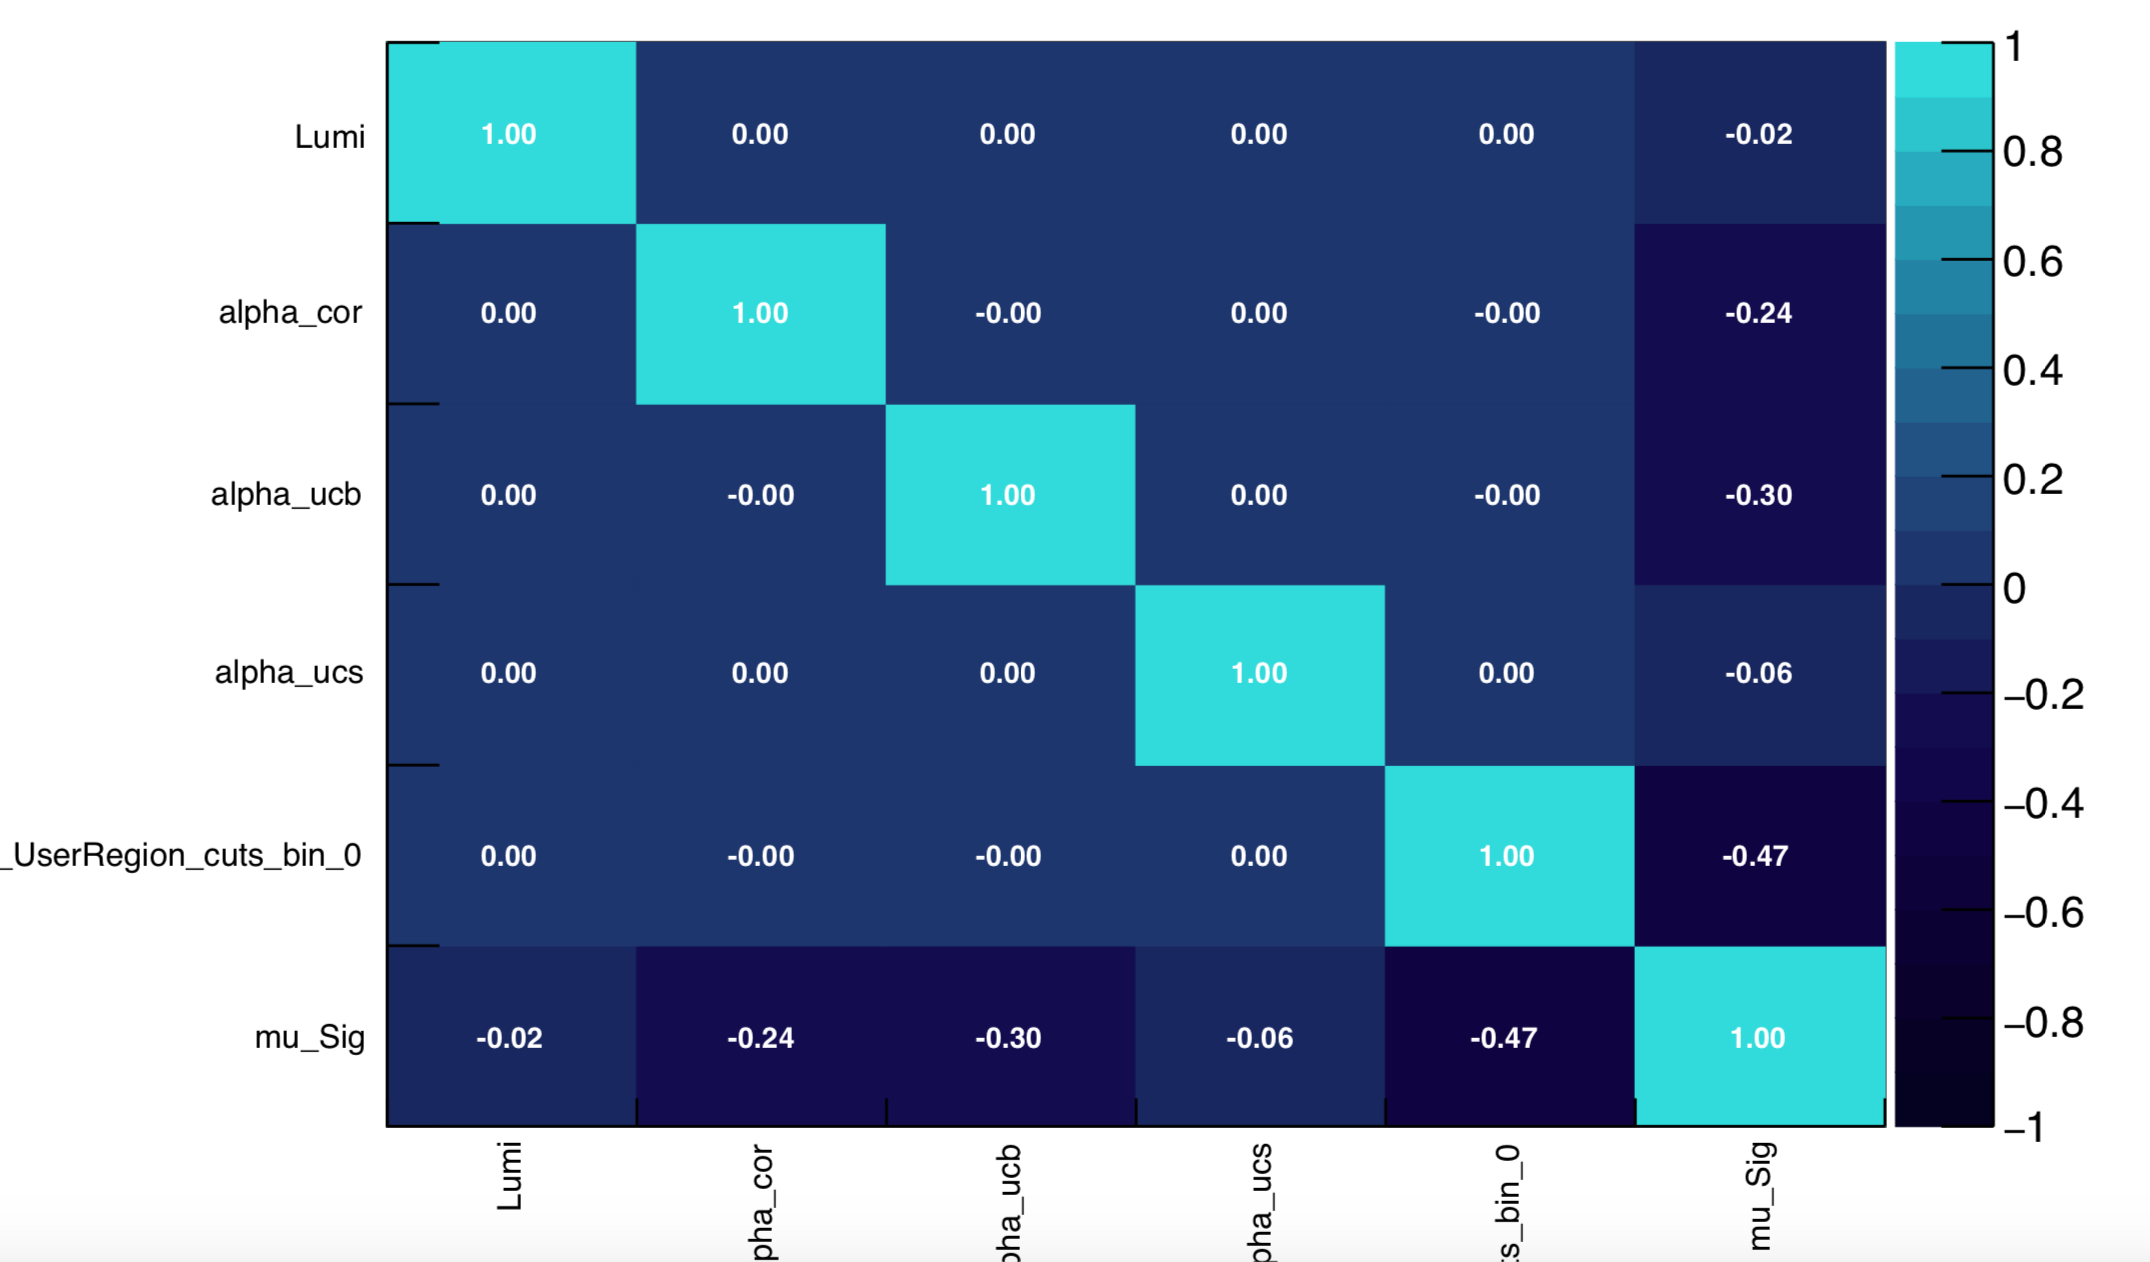
\includegraphics[width=0.65\textwidth]{correlationmatrix}
\end{figure}
\end{frame}

\end{document}
